\paragraph{4. Do the lost relations result in New Observable Behaviors?}

    To address this, we divide our cases into two parts; one for each type of relation lost:
    \begin{tasks}(2)
        \task $\reln{k}{hb}{W_{uo}}.$
        \task $\reln{W_{uo}}{hb}{k}.$
    \end{tasks}

    Figure~\ref{elim_write:case1} shows a breakdown of sub-cases for case (a), varying based
    on the nature of event $k$.
    \begin{figure}[H]
        \centering
        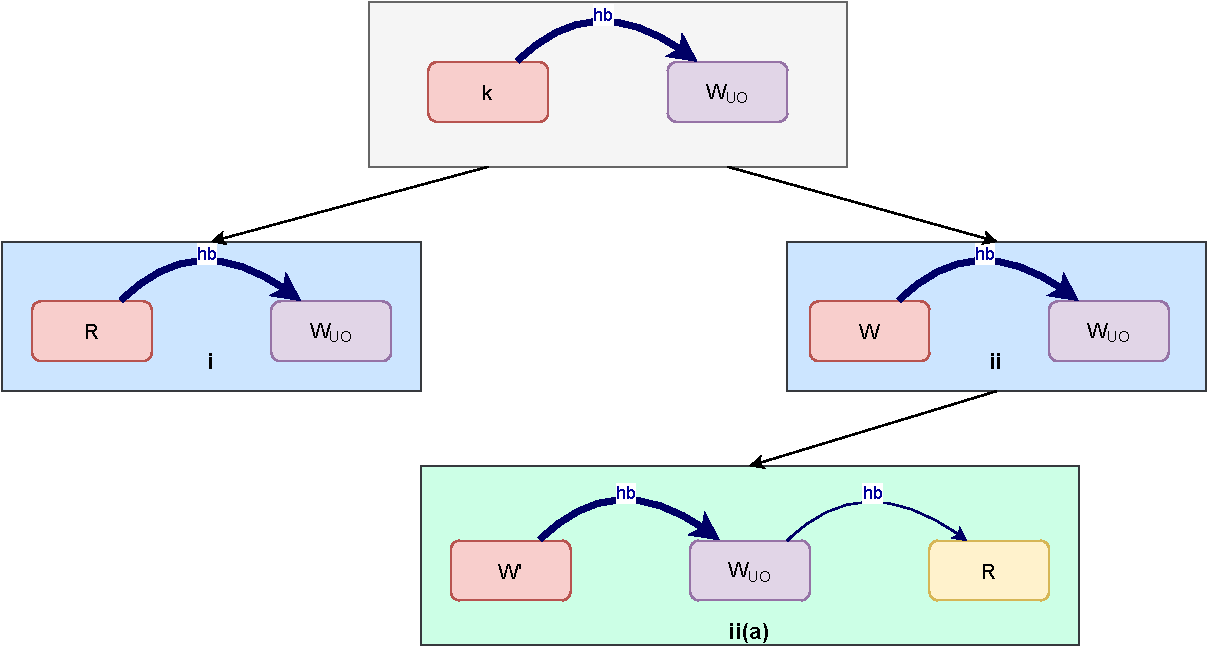
\includegraphics[scale=0.5]{6.Elimination/1.ValidEliminationCandidate/WriteElimProof/ProofParts/Part4Case1.pdf}
        \caption{The impact of lost relation $\reln{k}{hb}{W_{uo}}$ on observable behaviors.}
        \label{elim_write:case1}
    \end{figure}

    We can observe the following:
    \begin{itemize}
        \item (i) is a pattern from Axiom \ref{CoRe} that restricts the read $R$ reading from $e$. This reads-from restriction will remain the same after elimination of $e$. 
        \item (ii)(a) is a pattern from Axiom \ref{CoRe}, forbidding $R$ to read some bytes of $W'$. 
        The set of byte-level restrictions will remain the same after elimination, if firstly we have 
        \begin{align*}
            \reln{d}{hb}{R} \wedge \reln{W}{hb}{d}.
        \end{align*}
        By Lemma \ref{Lemma2}, the first relation holds and by Def of happens-before, the second will hold. 
        Secondly, we need to ensure that after elimination, Axiom \ref{CoRe} now restricts the exact set of $\stck{_{rbf}}$ relations with $W'$ and $R$ as before. 
        Since $R$ or $W'$ can be arbitrary, we would need the ranges of $e$ and $d$ to be same (i.e $\Re(e) = \Re(d)$).
    \end{itemize}

    Figure~\ref{elim_write:case2} shows a breakdown of sub-cases for case (b), varying based
    on the nature of event $k$.
    \begin{figure}[H]
        \centering
        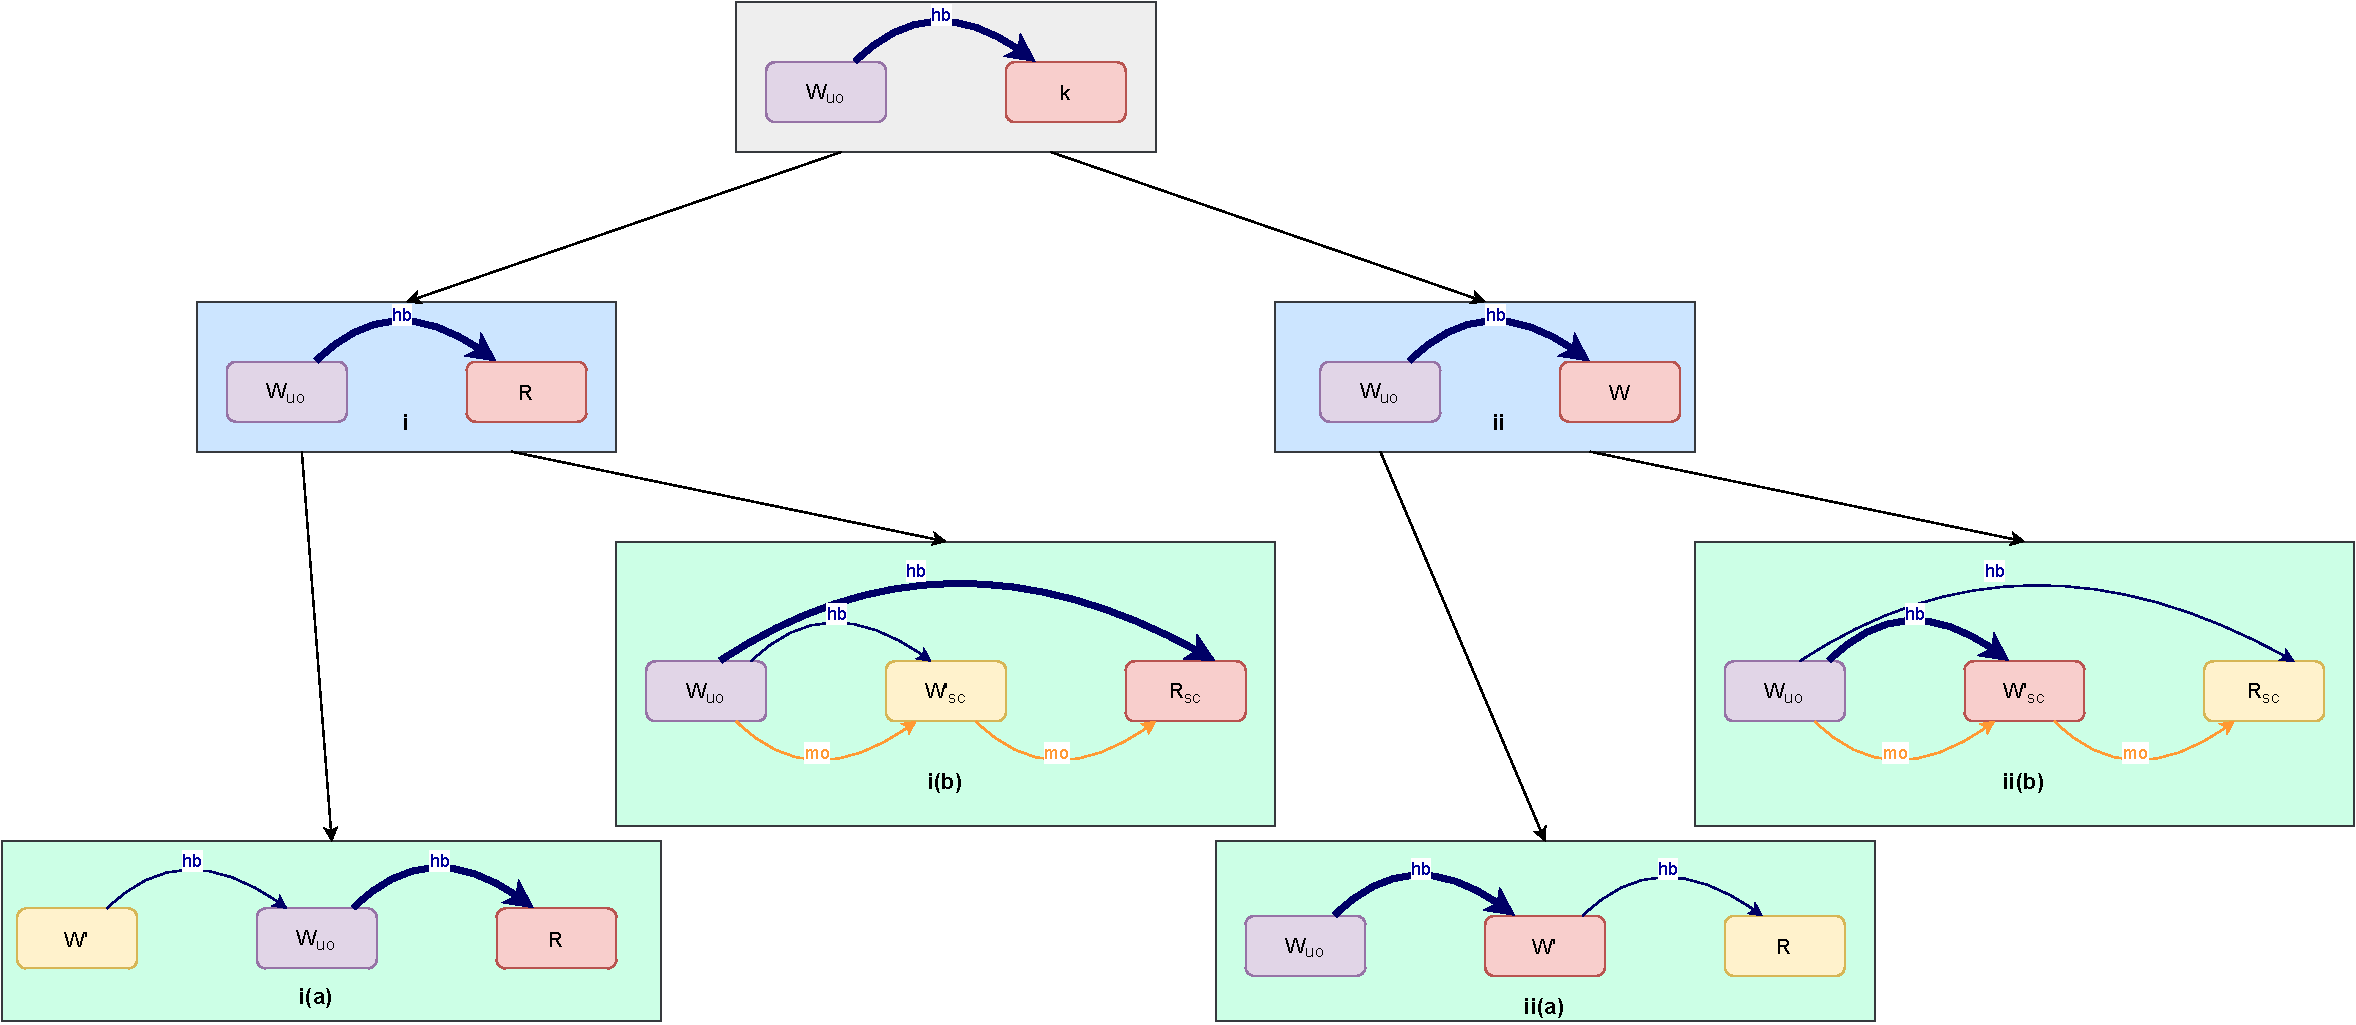
\includegraphics[scale=0.3]{6.Elimination/1.ValidEliminationCandidate/WriteElimProof/ProofParts/Part4Case2.pdf}
        \caption{The impact of lost relation $\reln{W_{uo}}{hb}{k}$ on observable behaviors.}
        \label{elim_write:case1}
    \end{figure}

    We make the following observations:
    \begin{itemize}
        \item (i)(a) has the similar argument to the previous case's (ii)(a), requiring $e$ and $d$ to have equal ranges.
        \item (i)(b) is a pattern from Axiom \ref{SeqCsAt}, which restricts $R$ from reading anything of $W$. This reads-from restriction will remain the same after $e$ is eliminated. 
        \item (ii)(a) is a pattern from Axiom \ref{CoRe}, restricting $R$ from reading $W$. This reads-from restriction will remain the same after after eliminating $e$.
        \item (ii)(b) is the same as (i)(b).
    \end{itemize}

    In all the above cases, we observe that on keeping range of $e$ and $d$ equal, none of the patterns introduce any new observable behavior. Hence, if we have two consecutive writes of equal ranges, of which the first one has access mode unordered, the set of Observable Behaviors without the write is a subset of that with it present. 